\documentclass[aspectratio=169, xcolor=dvipsnames]{beamer}

% --- Theme Setup ---
\usetheme{Madrid}
\usecolortheme{default}

% --- Packages ---
\usepackage{listings}
\usepackage{xcolor}
\usepackage{tikz}
\usetikzlibrary{shapes, arrows, positioning, fit, er} % Added 'er' library for ER diagrams
\usepackage{booktabs}
\usepackage{tcolorbox}
\usepackage{amsmath}
\usepackage{hyperref}

% --- Code Highlighting Style ---
\definecolor{codegreen}{rgb}{0,0.6,0}
\definecolor{codegray}{rgb}{0.5,0.5,0.5}
\definecolor{codepurple}{rgb}{0.58,0,0.82}
\definecolor{backcolour}{rgb}{0.95,0.95,0.92}

\lstdefinestyle{mystyle}{
    backgroundcolor=\color{backcolour},   
    commentstyle=\color{codegreen},
    keywordstyle=\color{magenta},
    numberstyle=\tiny\color{codegray},
    stringstyle=\color{codepurple},
    basicstyle=\ttfamily\footnotesize,
    breakatwhitespace=false,         
    breaklines=true,                 
    captionpos=b,                    
    keepspaces=true,                 
    numbers=left,                    
    numbersep=5pt,                  
    showspaces=false,                
    showstringspaces=false,
    showtabs=false,                  
    tabsize=2,
    escapechar=|
}
\lstset{style=mystyle}

% --- Notes Setup ---
\setbeameroption{hide notes} 

% --- Title Information ---
\title[DBMS - Unit 2]{Unit 2: ER Model and Relational Algebra}
\subtitle{Lecture 1: Introduction to ER Model \& Basic Concepts}
\author{Milav Dabgar}
\institute{Diploma in ICT}
\date{\today}

\begin{document}

% ==========================================
% Title Slide
% ==========================================
\begin{frame}
    \titlepage
\end{frame}

% ==========================================
% Table of Contents
% ==========================================
\begin{frame}{Table of Contents}
    \tableofcontents
\end{frame}

% ==========================================
% SECTION 1: Introduction
% ==========================================
\section{Introduction to Database Design}

\begin{frame}
  \vfill
  \centering
  \begin{beamercolorbox}[sep=8pt,center,shadow=true,rounded=true]{title}
    \usebeamerfont{title}Introduction to Database Design\par%
  \end{beamercolorbox}
  \vfill
\end{frame}

\begin{frame}{Why Conceptual Design?}
    \begin{block}{The Need for Design}
    Before implementing a database in a specific software (like MySQL or Oracle), we need a high-level blueprint.
    \end{block}
    
    \vspace{1em}
    
    \begin{itemize}
        \item \textbf{Communication Tool:} Bridges the gap between technical developers and non-technical stakeholders.
        \item \textbf{Blueprint:} Serves as a clear plan, similar to an architect's blueprint for a building.
        \item \textbf{Independence:} Focuses on \textit{what} data is stored, not \textit{how} it is implemented technically.
    \end{itemize}
\end{frame}

\begin{frame}{Limitations of File Systems}
    Why do we move towards Database Management Systems (DBMS)?
    
    \vspace{1em}
    
    \begin{alertblock}{File System Issues}
    \begin{itemize}
        \item \textbf{Data Redundancy:} Same data stored in multiple places.
        \item \textbf{Data Inconsistency:} Updates might not reflect everywhere.
        \item \textbf{Difficulty in Access:} Writing new programs for every new query is inefficient.
        \item \textbf{Security Problems:} Hard to enforce granular access constraints.
    \end{itemize}
    \end{alertblock}
    
    \vspace{0.5em}
    \textbf{Solution:} Structured Database Design using models like the ER Model.
\end{frame}

\begin{frame}{Where ER Model Fits}
    The ER model is used at the \textbf{Conceptual Level} of Database Abstraction.
    
    \vspace{2em}
    \centering
    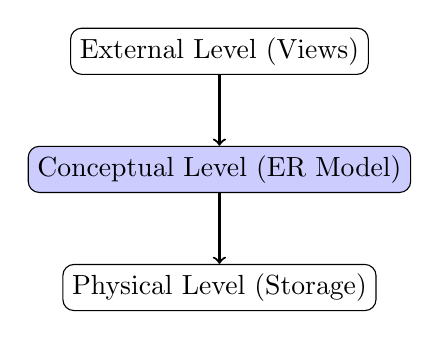
\begin{tikzpicture}[node distance=1.5cm, auto]
        \node (ext) [draw, rectangle, rounded corners] {External Level (Views)};
        \node (con) [draw, rectangle, rounded corners, fill=blue!20, below of=ext] {Conceptual Level (ER Model)};
        \node (phy) [draw, rectangle, rounded corners, below of=con] {Physical Level (Storage)};
        
        \draw[->, thick] (ext) -- (con);
        \draw[->, thick] (con) -- (phy);
    \end{tikzpicture}
\end{frame}

% ==========================================
% SECTION 2: ER Model Basics
% ==========================================
\section{ER Model Concepts}

\begin{frame}
  \vfill
  \centering
  \begin{beamercolorbox}[sep=8pt,center,shadow=true,rounded=true]{title}
    \usebeamerfont{title}ER Model: Basic Concepts\par%
  \end{beamercolorbox}
  \vfill
\end{frame}

\begin{frame}{What is the ER Model?}
    \begin{definition}[Entity-Relationship (ER) Model]
    A conceptual data model that views the real world as a collection of basic objects, called \textbf{entities}, and relationships among these objects.
    \end{definition}
    
    \vspace{1em}
    It is represented graphically using \textbf{Entity-Relationship Diagrams (ER Diagrams)}.
    
    \vspace{1em}
    \textbf{Key Components:}
    \begin{enumerate}
        \item Entities
        \item Attributes
        \item Relationships
    \end{enumerate}
\end{frame}

% ==========================================
% SECTION 3: Entities
% ==========================================
\section{Entities}

\begin{frame}{Entity and Entity Set}
    \begin{columns}
        \begin{column}{0.6\textwidth}
            \begin{block}{Entity}
            A "thing" or "object" in the real world that is distinguishable from other objects.
            \begin{itemize}
                \item \textit{Example:} A specific student (e.g., Milav), a specific car.
            \end{itemize}
            \end{block}
            
            \begin{block}{Entity Set}
            A set of entities of the same type that share the same properties.
            \begin{itemize}
                \item \textit{Example:} The set of all Students, the set of all Courses.
            \end{itemize}
            \end{block}
        \end{column}
        
        \begin{column}{0.4\textwidth}
            \centering
            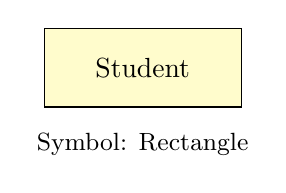
\begin{tikzpicture}
                % Entity Rectangle
                \node (entity) [draw, rectangle, minimum width=2.5cm, minimum height=1cm, fill=yellow!20] {Student};
                \node [below=0.2cm of entity] {\small Symbol: Rectangle};
            \end{tikzpicture}
        \end{column}
    \end{columns}
\end{frame}

\begin{frame}{Strong Entity}
    \begin{itemize}
        \item An entity that has a primary key (a unique identifier) is called a **Strong Entity**.
        \item It does not depend on any other entity for its existence.
    \end{itemize}
    
    \vspace{2em}
    
    \textbf{Examples:}
    \begin{itemize}
        \item \textbf{Student:} Identified by \textit{Enrollment No}.
        \item \textbf{Employee:} Identified by \textit{Employee ID}.
        \item \textbf{Course:} Identified by \textit{Course Code}.
    \end{itemize}
\end{frame}

% ==========================================
% SECTION 4: Attributes
% ==========================================
\section{Attributes}

\begin{frame}{Attributes}
    \begin{columns}
        \begin{column}{0.6\textwidth}
            \begin{definition}
            Attributes describe the properties or characteristics of an entity.
            \end{definition}
            
            \vspace{1em}
            \textit{Example:}
            For a \textbf{Student} entity, attributes could be:
            \begin{itemize}
                \item Name
                \item Enrollment No
                \item Date of Birth
                \item Mobile Number
            \end{itemize}
        \end{column}
        
        \begin{column}{0.4\textwidth}
            \centering
            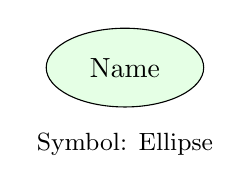
\begin{tikzpicture}
                % Attribute Oval
                \node (attr) [draw, ellipse, minimum width=2cm, minimum height=1cm, fill=green!10] {Name};
                \node [below=0.2cm of attr] {\small Symbol: Ellipse};
            \end{tikzpicture}
        \end{column}
    \end{columns}
\end{frame}

\begin{frame}{Types of Attributes}
    Attributes are classified based on their nature:
    
    \vspace{1em}
    \begin{enumerate}
        \item \textbf{Simple vs. Composite}
        \item \textbf{Single-valued vs. Multi-valued}
        \item \textbf{Stored vs. Derived}
        \item \textbf{Null Attributes}
    \end{enumerate}
\end{frame}

\begin{frame}{Simple vs. Composite Attributes}
    \begin{columns}[t]
        \begin{column}{0.48\textwidth}
            \textbf{Simple Attribute}
            \begin{itemize}
                \item Cannot be divided into smaller parts.
                \item \textit{Ex:} Enrollment No, Gender.
            \end{itemize}
        \end{column}
        
        \begin{column}{0.48\textwidth}
            \textbf{Composite Attribute}
            \begin{itemize}
                \item Can be divided into sub-parts (other attributes).
                \item \textit{Ex:} Name (First Name, Middle Name, Last Name).
                \item \textit{Ex:} Address (Street, City, State, Zip).
            \end{itemize}
        \end{column}
    \end{columns}
    
    \vspace{1em}
    \centering
    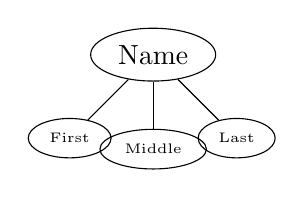
\begin{tikzpicture}[node distance=1.5cm]
        \node (name) [draw, ellipse] {Name};
        \node (first) [draw, ellipse, below left of=name, font=\tiny] {First};
        \node (middle) [draw, ellipse, below of=name, font=\tiny, node distance=1.2cm] {Middle};
        \node (last) [draw, ellipse, below right of=name, font=\tiny] {Last};
        
        \draw (name) -- (first);
        \draw (name) -- (middle);
        \draw (name) -- (last);
    \end{tikzpicture}
\end{frame}

\begin{frame}{Single-valued vs. Multi-valued Attributes}
    \begin{columns}[t]
        \begin{column}{0.48\textwidth}
            \textbf{Single-valued}
            \begin{itemize}
                \item Holds only one value for an entity.
                \item \textit{Ex:} Date of Birth, Enrollment No.
            \end{itemize}
        \end{column}
        
        \begin{column}{0.48\textwidth}
            \textbf{Multi-valued}
            \begin{itemize}
                \item Can hold multiple values for an entity.
                \item Represented by a \textbf{double ellipse}.
                \item \textit{Ex:} Mobile Number (a person can have two numbers), Degrees.
            \end{itemize}
        \end{column}
    \end{columns}
    
    \vspace{1em}
    \centering
    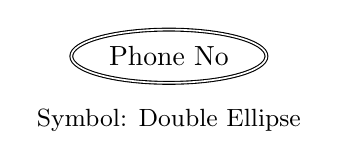
\begin{tikzpicture}
        \node (phone) [draw, ellipse, double, fill=white] {Phone No};
        \node [below=0.2cm of phone] {\small Symbol: Double Ellipse};
    \end{tikzpicture}
\end{frame}

\begin{frame}{Derived Attributes}
    \begin{itemize}
        \item Value is derived from another attribute.
        \item Not physically stored in the database, calculated when needed.
        \item Represented by a \textbf{dashed ellipse}.
    \end{itemize}
    
    \vspace{1em}
    \centering
    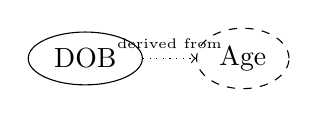
\begin{tikzpicture}[node distance=2cm]
        \node (dob) [draw, ellipse] {DOB};
        \node (age) [draw, ellipse, dashed, right of=dob] {Age};
        
        \draw[->, dotted] (dob) -- (age) node[midway, above, font=\tiny] {derived from};
    \end{tikzpicture}
\end{frame}

\begin{frame}{Lecture Summary}
    \begin{enumerate}
        \item \textbf{ER Model:} A blueprint for designing databases at the conceptual level.
        \item \textbf{Entity:} Real-world object (Rectangle).
        \item \textbf{Attribute:} Property of an entity (Ellipse).
        \item \textbf{Attribute Types:}
            \begin{itemize}
                \item Composite (Tree structure)
                \item Multi-valued (Double Ellipse)
                \item Derived (Dashed Ellipse)
            \end{itemize}
    \end{enumerate}
    
    \vspace{1em}
    \begin{center}
        \textit{Next Lecture: Relationships and Constraints}
    \end{center}
\end{frame}

\end{document}
